\section{引言}
\label{sec:intro}

\subsection{研究背景与问题定位}

飞行器的姿态与平动控制可以来自气动舵面、旋翼差速、推力矢量或它们的组合。
固定翼形态通常依赖副翼、升降舵和方向舵，舵面偏转改变当地翼型的有效弯度，产生附加气动力，经力臂形成控制力矩。
这一范式在常规飞行包线内成熟可靠，经历了一个多世纪的工程验证，现代民航客机和高性能战斗机均以此为基础\cite{stevens2015aircraft}。

然而，气动舵面控制存在若干无法回避的物理局限。其一，舵面控制效能随动压（$\propto V^2$）衰减——
在起飞滑跑初期和着陆拉平阶段，舵面偏转产生的力矩可能不足以克服扰动或执行机动指令。
其二，舵面偏转不可避免地产生附加阻力，降低巡航效率。
其三，大迎角下翼面流动分离导致舵面浸没在分离区内，舵效骤降甚至出现反效——这是失速/尾旋事故的重要诱因。

多旋翼飞行器的兴起提供了另一种思路：通过电机转速差动直接产生控制力矩，彻底摆脱对气动舵面的依赖\cite{mahony2012multirotor}。
多旋翼在悬停和低速段的操控性远超固定翼——每个旋翼既是升力源又是控制执行器，控制带宽不受动压限制。
然而，多旋翼的续航和速度性能远逊于固定翼，这是由桨盘载荷与气动效率的根本差异决定的。
固定翼巡航与旋翼悬停采用不同的效率指标，升阻比与悬停品质因数不能直接作数值比较。
从任务能耗看，固定翼以机翼升力承担重量，旋翼悬停则需持续向下加速空气；两者的诱导功率、盘载和飞行速度
共同决定续航差异，应在统一任务剖面下比较，而不能由两个异类无量纲指标直接推出结论。

矢量推力（thrust vectoring）技术作为第三种范式，通过改变发动机喷流（或螺旋桨滑流）方向来产生直接力矩。
该技术在军用航空领域已有成熟应用——如F-22的二元推力矢量喷管和Su-35的三元推力矢量喷管，
能够在失速后（post-stall）保持可控性，完成常规飞机无法实现的超机动动作\cite{stevens2015aircraft}。
其物理本质是：不依赖气动面与来流的相互作用，而是通过动量通量的方向偏转直接产生力和力矩。

将矢量推力概念引入小型电推进飞行器，结合多旋翼的差速控制思想（利用反扭矩差动产生偏航力矩），
可望形成纵列双发矢量推力布局。该构型的核心特征在于：
\textbf{正交摆轴使零摆角附近的三个力矩主通道呈置换后的近对角结构}，
因而可将通用过驱动平台的约束优化问题缩减为固定维数的局部矩阵分配问题
\cite{johansen2013control}。这种几何结构降低了分配复杂度，但反扭矩投影、有限摆角、
电机动态和执行器饱和仍会产生交叉耦合；当前固件仍在线构造并求逆$3\times3$效能矩阵。

\subsection{现有构型的分类与定位}

为理解本构型的创新点，有必要对现有矢量推力/垂直起降构型作简要分类。从推力方向的可控性角度，
可将电推进飞行器分为以下几类：

\textbf{固定推力方向}：所有常规固定翼和多旋翼均属此类。推力方向固连于机体，姿态控制通过
气动舵面（固定翼）或差速（多旋翼）实现。结构简单、可靠性高，但低速段控制权限受限（固定翼）
或巡航效率低（多旋翼）。

\textbf{倾转旋翼/倾转机翼}：V-22 Osprey和AW609为代表。旋翼短舱或整个机翼可倾转，
在垂直起降和高速巡航之间切换。倾转机构复杂、重量代价大，且倾转过渡段的控制律设计
（增益调度或非线性控制）具有相当的理论与工程难度\cite{kang2009control}。

\textbf{通用多自由度矢量推力}：每个推进器可在两个方向独立倾斜（如万向节悬挂），
$n$个推进器产生极大的执行空间冗余，控制分配为欠定问题\cite{seguigasco2014novel}。
这类构型灵活性极高，理论上可实现任意方向平动和姿态的独立控制，
但代价是机械复杂度高（每个推进器需两套伺服机构）、控制分配需要在线求解优化问题、
且多个推进器之间的气动干扰效应复杂\cite{zhu2025experimental}。

\textbf{纵列双发正交单轴矢量推力（本文构型）}：每个推进器仅有一个摆动自由度，
两摆轴正交，加上差速通道，总计四个执行器恰好控制四个主自由度（总推力+三轴力矩）。
摆轴正交使推力力臂主项形成对角结构，但反扭矩投影仍保留一阶交叉项。
该构型不以机翼为必要条件，而是以双推进器和摆座作为基础平台，按任务形成不同形态：
安装横向机翼时，机翼可在前飞段承担主要气动升力，构成固定翼巡航形态；
不安装机翼时，推进器可在竖直姿态下承担主要升力，形成类似多轴飞行器的垂起、悬停和低速机动形态；
在两者之间还可研究机翼安装状态、姿态和推力方向共同变化的过渡形态。
因此本文将其定位为\textbf{模块化、多形态矢量推力飞行器}，而非仅限于固定翼或tail-sitter平台。

\subsection{构型概念与形态模式}
\label{sec:configuration_modes}

本文研究的是一个以双推进器矢量推力机构为核心、可选配不同气动外形的模块化平台。
机翼不是推进与姿态控制成立的必要条件，而是影响升力分担、航程效率和过渡特性的任务模块。
构型由以下核心要素和工作形态构成：

\begin{enumerate}[label=(\arabic*)]
    \item \textbf{纵列双发}：两台电机沿机体纵轴（$x_b$）前后布置。前电机为拉力式
          （tractor），螺旋桨位于重心前方；尾电机为推进式（pusher），
          螺旋桨位于重心后方。双发沿纵轴布置最大限度地利用了机身长度作为摆动力臂；
    \item \textbf{反向旋转}：前后螺旋桨旋向相反，使名义等转速、零摆角工作点的轴向
          反扭矩近似抵消。只有在转子角动量、摆角、入流与转速响应近似对称时，
          部分陀螺交叉项才会同步减弱；P-factor受前进比、迎角与局部入流影响，
          不能仅凭反向旋转笼统判定为消失。旋向正负在第\ref{sec:mapping}节用有符号变量定义，
          避免观察方向造成CW/CCW歧义；
    \item \textbf{正交单轴摆座}：在推进模型系$\{P\}$中，前电机绕$z'$轴摆动，尾电机绕
          $y'$轴摆动。两摆轴正交，使两者分别产生$M_{z'}$与$M_{y'}$主力矩；
          映射到固件任务系后，对应上摆滚转与下摆俯仰。反扭矩投影仍产生一阶交叉项，
          因而应称为主通道近似解耦；
    \item \textbf{差速反扭力矩}：打破两发电机的反扭矩平衡（通过差速指令$\Delta\omega$
          使一台加速、另一台减速），产生推进模型系$x'$轴净力矩；经固件轴置换后，
          该通道承担悬停任务语义中的偏航主控。这一机制本质上是反向旋转推进器
          扭矩差控制原理在纵列布局上的应用。
\end{enumerate}

在上述基础机构之上，定义四种研究形态：
\begin{enumerate}[label=(\alph*)]
    \item \textbf{有翼前飞形态}：安装横向机翼，机翼在中高速前飞时承担主要升力，
          推进器提供前向推进，矢量推力和气动舵面可按控制分配共同工作；
    \item \textbf{无翼垂起形态}：拆除机翼或采用弱气动升力机身，飞行器在竖直姿态下由双推进器承担主要升力，
          通过摆座和反扭差速实现类似多轴飞行器的悬停、平移和姿态控制；
    \item \textbf{有翼垂起形态}：保留机翼并采用竖直姿态起降，机翼在悬停段主要作为结构和附加气动部件，
          在前飞后逐步接管升力；
    \item \textbf{形态过渡}：在有翼/无翼配置、机体姿态、推力方向和气动升力共同变化时，
          需要进行模式调度、参数切换和控制权限平滑交接。本文当前仿真重点验证单一形态的局部动力学，
          连续过渡仍属于后续扩展内容。
\end{enumerate}

该构型的核心设计哲学是：\textbf{用几何设计换取算法简洁性，并用模块化形态扩展任务包线}。
在通用矢量推力平台中，控制分配是$6 \times 3n$的欠定优化问题，需要在线求解伪逆或二次规划；
在本构型中，正交摆轴的几何约束将姿态执行空间维数降至与三个力矩目标相同，
零摆角附近可采用三通道直接映射作为低复杂度近似；当前固件为处理交叉项和工作点变化，
采用在线$3\times3$效能矩阵求逆，并在输出端处理摆角、差速和单侧转速限幅。

\begin{figure}[H]
\centering
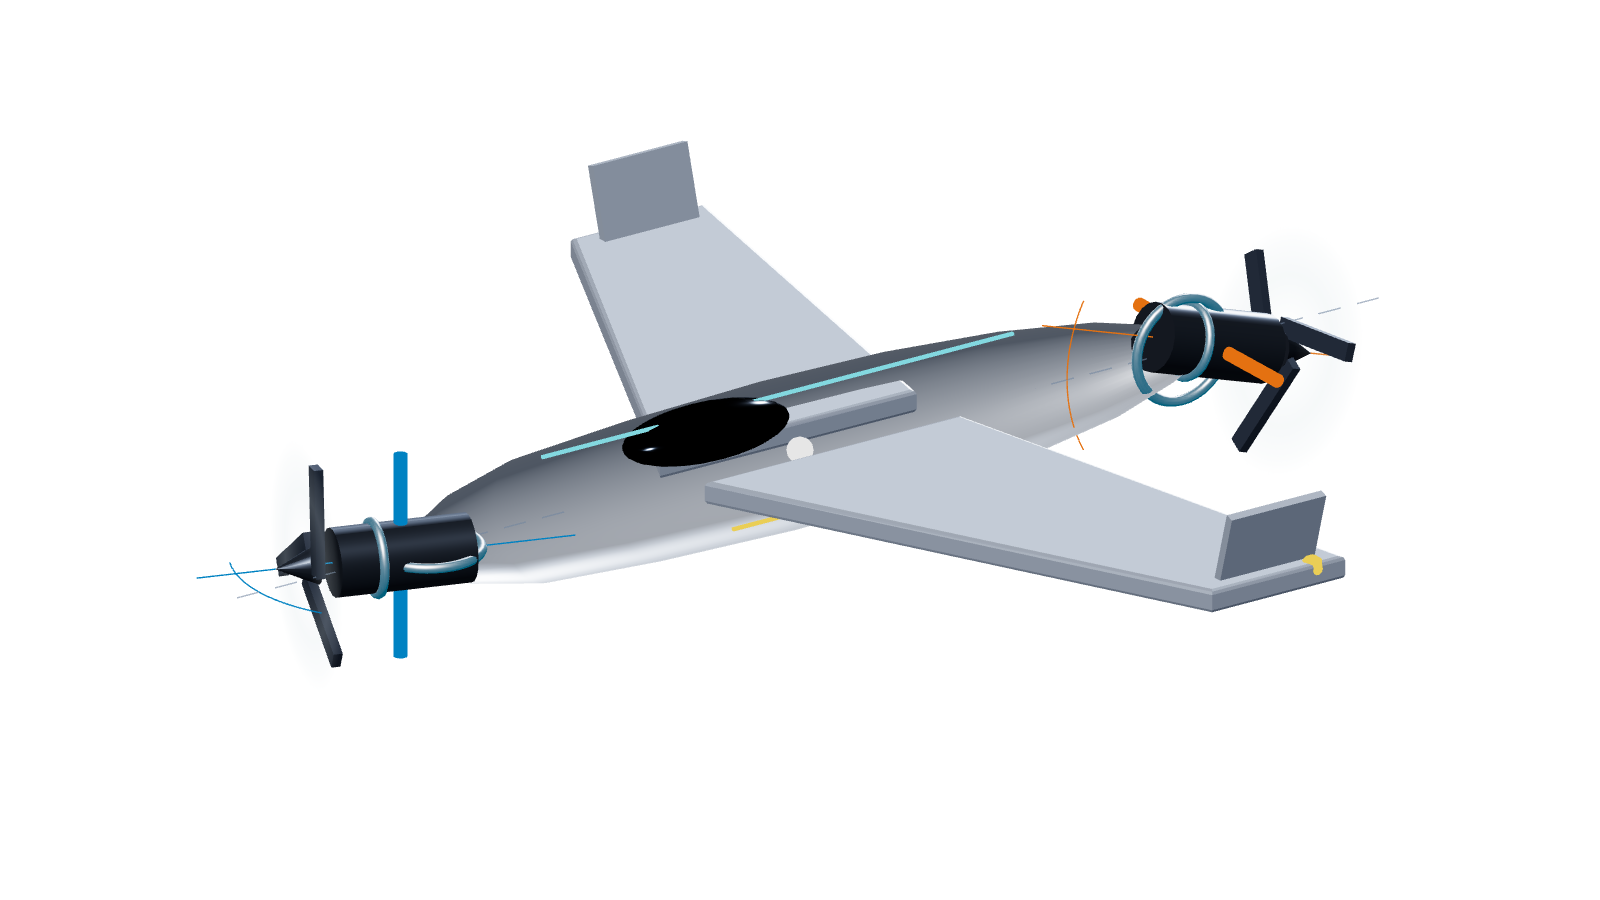
\includegraphics[width=0.99\linewidth]{fig/01-web-orthogonal-deflection.png}
\caption{纵列双发正交单轴矢量推力构型的程序化几何快照。前、尾摆座分别给出
$\delta_f=+18^\circ$ 与 $\delta_t=+18^\circ$ 的辨识姿态，用于显示两个正交摆动平面；
该姿态不是配平或标定工作点。渲染几何不按工程尺度，物理力臂以参数源中的
$a=b=0.315\,\mathrm{m}$为准。推进模型系的力和力矩方向见\cref{fig:thrust_mapping}。}
\label{fig:configuration}
\end{figure}


\subsection{坐标系、轴置换与控制语义（2026-08-07 轴置换后）}
\label{sec:axis_semantics}

早期稿件混用了理论推进模型坐标与飞控安装坐标，这是“前摆偏航/差速滚转”和
“上摆滚转/差速偏航”两种说法并存的根源。本文将两套坐标明确分离：理论推进模型采用
$\{P\}$系，其$x'$轴沿名义推力轴，$y'$轴对应下摆力矩主轴，$z'$轴对应上摆力矩主轴；
飞控采用固件FRD任务系$\{F\}$。2026年8月7日实机轴置换后，两者满足
\begin{equation}
    \begin{bmatrix} M_{x'} \\ M_{y'} \\ M_{z'} \end{bmatrix}
    =
    \underbrace{\begin{bmatrix}
        0 & 0 & -1 \\
        0 & 1 & 0 \\
        1 & 0 & 0
    \end{bmatrix}}_{\mathbf{R}_{P\leftarrow F}}
    \begin{bmatrix} M_x^F \\ M_y^F \\ M_z^F \end{bmatrix},
    \qquad x'=-z_F,\;y'=y_F,\;z'=x_F .
    \label{eq:frame_permutation}
\end{equation}
该矩阵是同一物理矢量在两套坐标中的分量变换，不是随飞行姿态改变轴的名称。
固件混控还叠加传感器安装与舵机标定符号，故字面指令映射应以
\texttt{flight\_control.cpp}的任务轴置换和执行器标定为准，不能只由
式\eqref{eq:frame_permutation}反推。

在$\{P\}$系中，执行器主效能始终为$\Delta\omega\rightarrow M_{x'}$、
$\delta_t\rightarrow M_{y'}$、$\delta_f\rightarrow M_{z'}$。结合轴置换与实机标定后，
飞行任务语义为\textbf{上摆$\delta_f$对应滚转、下摆$\delta_t$对应俯仰、
差速$\Delta\omega$对应偏航}。后文讨论力与力矩公式时均采用$\{P\}$系分量；
讨论飞行员指令、姿态环或实机通道时采用$\{F\}$系滚转/俯仰/偏航语义。

\subsection{本文结构}

本文按从底层物理到顶层控制的逻辑链展开：
第\ref{sec:propulsion}节建立推进系统的集总参数模型，从桨盘动量理论出发推导推力与反扭矩的相似律，
并分析电机动态和陀螺效应的物理机制；
第\ref{sec:mapping}节导出摆座运动学，给出完整的六维力/力矩映射，分离主控项与耦合项；
第\ref{sec:dynamics}节建立整机六自由度刚体动力学方程，包括牛顿-欧拉方程、四元数姿态运动学及数值积分策略；
第\ref{sec:allocation}节分析控制效能矩阵的对角化性质，评估耦合项的量级，并与通用推力矢量平台进行对比；
第\ref{sec:stability}节进行小扰动线性化，分析纵向和横航向各飞行模态的物理特性；
第\ref{sec:control}节设计级联式增稳控制律框架，给出各通道SAS律的整定原则；
第\ref{sec:discussion}节系统讨论构型的优势、已知局限、设计权衡及扩展方向。

在基础主线之上，本文以\textbf{主算法优先}的叙事组织控制部分：
第\ref{sec:quat_control}节建立误差四元数姿态表示（主算法外环的理论基础），
第\ref{sec:vtol}节给出 Tail-sitter 悬停应用场景，
第\ref{sec:cascade_chapter}节提出\textbf{级联姿态-角速度控制架构}——
本文的\textbf{主算法}（NDI 式：模型逆 + 前馈对消 + 在线效能矩阵分配，已实机上线），
第\ref{sec:simulation}节对主算法进行数值仿真验证；
其后第\ref{sec:INDI}、\ref{sec:lqr}节及自抗扰（第\ref{sec:online_id}章相关）、
模型预测控制（第\ref{sec:mpc}章）为\textbf{扩展/对比方案}，
以主算法为基准讨论其增强潜力与适用边界，最后回到第\ref{sec:discussion}节的讨论与
第\ref{sec:conclusion}节的结论。
